%==============================================================================
% Sjabloon poster bachproef
%==============================================================================
% Gebaseerd op document class `a0poster' door Gerlinde Kettl en Matthias Weiser
% Aangepast voor gebruik aan HOGENT door Jens Buysse en Bert Van Vreckem

\documentclass[a0,portrait]{hogent-poster}

% Info over de opleiding
\course{Bachelorproef}
\studyprogramme{toegepaste informatica}
\academicyear{2024-2025}
\institution{Hogeschool Gent, Valentin Vaerwyckweg 1, 9000 Gent}

% Info over de bachelorproef
\title{Optimalisatie van back-upstrategieën voor Azure PostgreSQL en MySQL databases bij Forvis Mazars met behulp van immutabele opslag en automatische back-ups: Een Proof-of-Concept.}
\author{Naoufal Bouazzaoui}
\email{naoufal.bouazzaoui@student.hogent.be}
\supervisor{Martijn Saelens}
\cosupervisor{Rémy Tetaert (Forvis Mazars)}

% Indien ingevuld, wordt deze informatie toegevoegd aan het einde van de
% abstract. Zet in commentaar als je dit niet wilt.
\specialisation{Systeem- en Netwerkbeheer}
\keywords{Back-ups, automatisatie, ransomware}

\begin{document}

\maketitle

\begin{abstract}
Dit onderzoek analyseert en optimaliseert de back-upstrategie van Forvis Mazars, met een focus op bescherming tegen ransomware-aanvallen. Het huidige systeem maakt gebruik van automatische full back-ups voor databases in Azure, maar herstelt ook onnodig alle databases bij een specifieke restore. Een Proof-of-Concept (PoC) in een lokale testomgeving met VirtualBox testte de effectiviteit van immutable storage, die back-ups beschermt tegen manipulatie, zelfs bij volledige controle van een aanvaller. Daarbij werd de back-upstrategie ook verbeterd door enerzijds immutable storage te implementeren in de Azure-productieomgeving en anderzijds de dagelijkse back-ups te automatiseren met behulp van Kubernetes cronjobs. Het herstelproces werd getest om de efficiëntie van het herstel te evalueren. Daarnaast werd een literatuurstudie uitgevoerd om technieken voor ransomware-resistentie en back-upstrategieën te onderzoeken.
\end{abstract}

\begin{multicols}{2} % This is how many columns your poster will be broken into, a portrait poster is generally split into 2 columns

\section*{Introductie}

In de digitale wereld van vandaag is gegevensbeveiliging een prioriteit. Ransomware-aanvallen bedreigen de integriteit van belangrijke gegevens, waardoor een robuuste back-upstrategie essentieel is voor snel herstel en bescherming tegen verlies.

\subsection*{Probleemstelling}  
De huidige back-upstrategie bij Forvis Mazars biedt een basisbescherming, maar vertoont tekortkomingen op het gebied van automatisering, beveiliging en herstelbaarheid. Er is weinig inzicht in de snelheid en betrouwbaarheid van het herstelproces, en de back-ups zijn niet goed beschermd tegen moderne bedreigingen zoals ransomware.

\subsection*{Hoofdonderzoeksvraag}  
Hoe kan de back-upstrategie voor Azure PostgreSQL en MySQL databases bij Forvis Mazars geoptimaliseerd worden door het gebruik van immutabele opslag en automatische back-ups?

\subsection*{Deelvragen}  
\begin{itemize}
    \item Hoe veilig en betrouwbaar zijn de huidige back-upoplossingen van Forvis Mazars voor Azure PostgreSQL en MySQL databases?
    \item Welke rol speelt immutable opslag in het beschermen van back-ups tegen ransomware?
    \item Wat zijn de belangrijkste uitdagingen bij het integreren van immutable opslag met Azure cloud back-upsystemen?
\end{itemize}

\section{Experimenten}

A newt? Camelot! Why? No, no, no! Yes, yes. A bit. But she's got a wart.

Shut up! I dunno. Must be a king. Who's that then? Look, my liege! On second thoughts, let's not go there. It is a silly place.

Shut up! Will you shut up?! No, no, no! Yes, yes. A bit. But she's got a wart. He hasn't got shit all over him. It's only a model. It's only a model.

Bring her forward! I don't want to talk to you no more, you empty-headed animal food trough water! I fart in your general direction! Your mother was a hamster and your father smelt of elderberries! Now leave 

\section{Sectie met figuur}

De {\LaTeX} figure-omgeving bepaalt zelf waar een afbeelding komt en dat is meestal niet op de plek in de tekst waar de figure-omgeving gedefinieerd wordt. Als je wilt forceren dat afbeeldingen toch in de flow van de tekst blijven, dan kan je dat zoals hieronder:

\begin{center}
  \captionsetup{type=figure}
  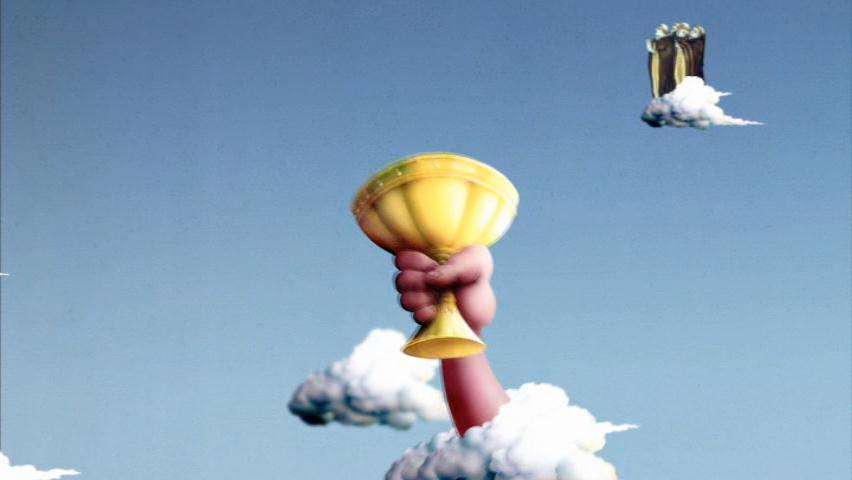
\includegraphics[width=1.0\linewidth]{grail}
  \captionof{figure}{He hasn't got shit all over him. The nose? Where'd you get the coconuts? What do you mean? We shall say `Ni' again to you, if you do not appease us}
\end{center}

Let er wel op dat dit tot problemen met bladschikking kan leiden.

\section{Conclusies}

Don't underestimate the Force. Oh God, my uncle. How am I ever gonna explain this? I suggest you try it again, Luke. This time, let go your conscious self and act on instinct. Don't be too proud of this technological terror you've constructed. The ability to destroy a planet is insignificant next to the power of the Force.

\section{Toekomstig onderzoek}

I care. So, what do you think of her, Han? No! Alderaan is peaceful. We have no weapons. You can't possibly… I have traced the Rebel spies to her. Now she is my only link to finding their secret base.

Kid, I've flown from one side of this galaxy to the other. I've seen a lot of strange stuff, but I've never seen anything to make me believe there's one all-powerful Force controlling everything. There's no mystical energy field that controls my destiny. It's all a lot of simple tricks and nonsense. You are a part of the Rebel Alliance and a traitor! Take her away! 

\end{multicols}
\end{document}